% !TeX root = main.tex
\documentclass[11pt,a4paper]{report}
%%%%%%%%%%%%%%%%%%%%
%   Package setup
%%%%%%%%%%%%%%%%%%%%

\usepackage{array}
\usepackage{tabularx}
\setlength {\marginparwidth }{2cm}
\usepackage{todonotes}
\usepackage{float}
\usepackage{tikz}
\usepackage{hyperref}

\usepackage{listings}

\usepackage[T1]{fontenc}
\usepackage{inconsolata}

\usepackage{color}

\definecolor{pblue}{rgb}{0.13,0.13,1}
\definecolor{pgreen}{rgb}{0,0.5,0}
\definecolor{pred}{rgb}{0.9,0,0}
\definecolor{pgrey}{rgb}{0.46,0.45,0.48}
\lstset{language=Java,
  showspaces=false,
  showtabs=false,
  breaklines=true,
  showstringspaces=false,
  breakatwhitespace=true,
  commentstyle=\color{pgreen},
  keywordstyle=\color{pblue},
  stringstyle=\color{pred},
  basicstyle=\ttfamily,
  moredelim=[il][\textcolor{pgrey}]{$$},
  moredelim=[is][\textcolor{pgrey}]{\%\%}{\%\%}
}
%%%%%%%%%%%%%%%%%%%%
%  Document setup
%%%%%%%%%%%%%%%%%%%%

\usepackage[includehead]{geometry}
\usepackage{fancyhdr}

%%%%%%%%%%%%%%%%%%%%
% Custom stuff below
%%%%%%%%%%%%%%%%%%%%

\def\checkmark{\tikz\fill[scale=0.4](0,.35) -- (.25,0) -- (1,.7) -- (.25,.15) -- cycle;} 

\def \jfun[#1]{
    {\tiny \textbf{(P. #1\footnote{Java Fundamentals})}}
}

\def \jdp[#1]{
    {\tiny \textbf{(P. #1\footnote{Java Design Patterns})}}
}
\author{Mikkel Helsing Andersen}
\title{Object Oriented Programming notes}

\begin{document}
    %%%%%%%%%%%%%%%%%%%%
    %  Document setup
    %%%%%%%%%%%%%%%%%%%%
    \pagestyle{fancy}
    \maketitle
    \tableofcontents\label{toc}
    \fancyhead{} % resets header
    \fancyhead[L]{OOP notes}
    \fancyhead[C]{\textbf{Mikkel Helsing Andersen}}
    \fancyhead[R]{AAU - DAT 3}
    \fancyfoot{} % resets footer
    \fancyfoot[L]{\hyperref[toc]{Table of Contents}}
    \fancyfoot[R]{\thepage}

    %%%%%%%%%%%%%%%%%%%%
    %     Content
    %%%%%%%%%%%%%%%%%%%%
    \chapter*{Programming concepts}
\begin{center}
    \textit{A programming paradigm is a way of conceptualizing what it means to perform
    computation, and how tasks that are to be carried out on a computer should be structured
    and organized.}
\end{center}

A program has two components data and algorithms.

\begin{list}{paradigm}{0.5cm}
    \item[Imperative paradigm:] Also know as algorithmic paradigm, think C. No classes, references to memory, sequentiel running of program/algorithm.
    \item[Procedural paradigm:] Same as Imperative except it's more modular, meaning code is easily reusable. 
    \item[Declarative paradig:] Computer finds the solution to a problem, think SQL. The data is "permanent".
    \item[Functional paradigm:] Based on mathematical functions. Data is immutable (Underlying structure cannot be changed). Java allows for lambda functions which allows for creating functional programming.
    \item[Logic paradigm:] Set the goal and specify the problem, to make the computer solve the problem, instead of writing an algorithm for finding said solution.
    \item[Object-oriented par:] Objects contains the data and algorithms. Where data is the state of the object. The algorithms allows to change the state of an object. Objects are often described as classes in programming. Think Java, C\# etc.
\end{list}
\clearpage
\section*{Polymorphism}
\subsection*{Overloading Polymorphism}
Multiple definition of a function with varying parameters.
\begin{figure}[h!]
    \begin{lstlisting}[language=Java]
    public class MathUtil {
        public static int max(int n1, int n2) {
            /*code*/
        }
        public static double max(double n1, double n2) {
            /*code*/
        }
        public static int max(int[] num) {
            /*code*/
        }
    }
    \end{lstlisting}
\end{figure}

\subsection*{Coercion Polymorphism}
When a type is implicitly converted.
\begin{figure}[h!]
    \begin{lstlisting}[language=Java]
    int num = 707;
    double d1 = (double)num; // Explicit
    double d2 = num; // Implicit
    \end{lstlisting}
\end{figure}

\subsection*{Inclusion Polymorphism}
Subtype, meaning a type/class that extends or implements a type/class can also be assigned to it's parent type. Think employee extends person can also be assigned to a variable with type person.
\clearpage
\subsection*{Parametric Polymorphism}
Lets classes and algorithms be generic without type specification
\begin{figure}[h!]
    \begin{lstlisting}[language=Java]
    List<String> sList = new ArrayList<String>();

    public <T> T example(T test) {
        return test;
    }

    class test<T> {
        /*code*/
    }
    \end{lstlisting}
\end{figure}

    \chapter{Classes}
Chapter begins: \jfun[225]

\section{What is a Java Class}
Java Classes has a set of properties and functionalities. Non-static classes can be instantiated. Classes can also work with generic types and inlusion as mentioned in \hyperref[sec:parametric_polymorphism]{polymorphism} and \hyperref[sec:inclusion_polymorphism]{inclusion respectivly}. Include the following:
\begin{itemize}
    \item Fields
    \item Methods
    \item Constructors
    \item Static initializers
    \item Instance initializers
\end{itemize}
Basis for creating a class:
\begin{lstlisting}[language=Java]
    // <T> is only for generic classes
    [modifiers] class class-name <T> {
        // Body of the class goes here
    }
    // Example
    public abstact class Human<T> {
        // An empty body for now
    }
\end{lstlisting}
Static fields in a class are class fields, whereas none static fields are instance variables.

\subsection*{Imports}
Import statements that uses the wild(*) modifier are on demand imports, meaning all available classes and functions can be used on demand:
\begin{lstlisting}[language=Java]
    import com.java.string.*
\end{lstlisting}
The Java compiler must resolve the simple name A to its fully qualified name during the compilation process. It searches for a type referenced in a program in the following order:
\begin{itemize}
    \item The current compilation unit
    \item Single-type import declarations
    \item Types declared in the same package
    \item Import-on-demand declarations
\end{itemize}

    \part{Design patterns}
\chapter{SOLID}
\begin{figure}[H]
    \centering
    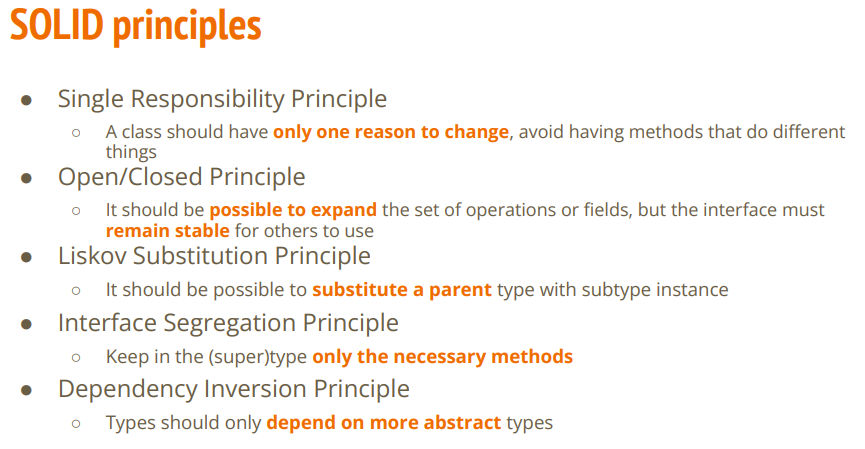
\includegraphics[width=\linewidth]{chapters/design_patterns/figures/solid.png}
\end{figure}
\chapter{Creational Patterns}
\section{Factory}
\begin{figure}[H]
    \centering
    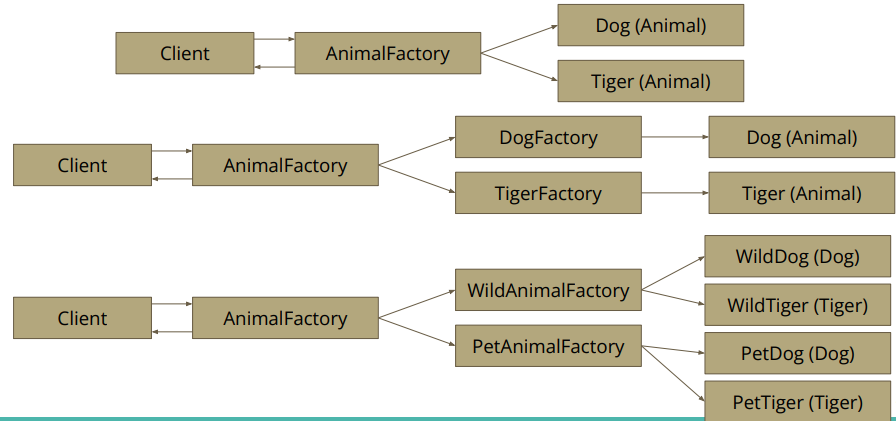
\includegraphics[width=\linewidth]{chapters/design_patterns/figures/factory_pattern_base.png}
\end{figure}
\clearpage
\subsection{Simple Factory}
\begin{lstlisting}
class AnimalFactory {
    public Animal createAnimal(Type animalType) {
        Animal animal = null;
        if (animalType.equals(Type.DOG)) {
            animal = new Dog();
        } else if (animalType.equals(Type.TIGER)) {
            animal = new Tiger();
        } else if (animalType.equals(Type.CAT)) {
            animal = new Cat();
        }
        return animal;
    }
}
         
\end{lstlisting}

\clearpage
\subsection{Factory Pattern}
An object with a method that creates new objects using abstraction.
\begin{lstlisting}
// Base factory
abstract class AnimalFactory {
    public abstract Animal createAnimal();
}

// One factory using the base factory
class DogFactory extends AnimalFactory {
    public Animal createAnimal() {
        return new Dog();
    }
}

// Usage of factory
AnimalFactory factory = new DogFactory();
Animal animal = factory.createAnimal();
animal.displayBehavior();
\end{lstlisting}

\clearpage
\subsection{Abstract Factory}
\begin{lstlisting}
// Base factory
interface AnimalFactory {
    Tiger createTiger();
    Dog createDog();
}

// Wild factory
public class WildAnimalFactory implements AnimalFactory {
    public Tiger createTiger() { ... }
    public Dog createDog() { ... }
}

// Pet factory
public class PetAnimalFactory implements AnimalFactory {
    public Tiger createTiger() { ... }
    public Dog createDog() { ... }
}

// Usage
AnimalFactory factory = new WildAnimalFactory();
Animal animal = factory.createTiger();
animal.displayBehavior();
\end{lstlisting}
\clearpage
\section{Builder Pattern}
\begin{lstlisting}
// Instantiating class at the beginning
public class Course {
    ...
    public static class CourseBuilder {
        private Course c;
        public CourseBuilder() {
            c = new Course();
        }
        public void setCode(String code); {
            c.code = code;
        }
        public void setTitle(String title) {
            c.title = title;
        }
        public Course getCourse() {
            return c;
        }
    }
}

// Using rigged constructor
public class Course {
    ...
    public static class CourseBuilder {
        private String ccode, ctitle;
        public CourseBuilder() { }
        public void setCode(String code) {
            ccode = code;
        }
        public void setTitle(String title) {
            ctitle = title;
        }
        public Course getCourse() {
            return new Course(ccode, ctitle);
        }
    }
}


\end{lstlisting}

\chapter{Structural Patterns}
\section{Decorator Pattern}
Dynamically add responsibilities to an object using composition. The decorator has the same interface as the decorated object, meaning it has the same interaction from the client perspective.

\begin{lstlisting}
abstract class Home {
    public double basePrice;
    public double additionalCost;
    
    public Home() {
        this.basePrice = 100000.0;
        this.additionalCost = 0.0;
    }

    public abstract double getPrice();
}

class BasicHome extends Home {
    @Override
    public double getPrice() {
        return this.basePrice;
    }
}

// Abstract class for creating decorators
abstact class Luxury extends Home {
    protected Home home;
    public double luxuryCost;

    public Luxury(Home home) {
        this.home = home;
    }

    @Override
    public double getPrice() {
        return this.home.getPrice();
    }
}

// Decorator
class SwimmingPool extends Luxury {
    public SwimmingPool(Home home) {
        super(home);
        this.luxuryCost = 20000;
    }

    @Override
    public double getPrice() {
        return this.home.getPrice() + this.luxuryCost;
    }
}

// Usage
Home home = new BasicHome;
home.getPrice() // Now 100000
// Add decorator to home
home = SwimmingPool(home);
home.getPrice() // Now 120000
\end{lstlisting}
\section{Adapter Pattern}
Adapts a class to conform to another class by creating a middleman layer that adapts it.
\subsection{Object adapter}
\begin{lstlisting}
interface RectInterface {
    void aboutMe();
}

class Rectangle implements RectInterface {
    ....
    @Override
    public void aboutMe() {
        System.out.println("I got 4 corners")
    }
}

interface TriInterface {
    void aboutTriangle();
}

class Triangle implements TriInterface {
    ....
    @Override
    public void aboutTriangle() {
        System.out.println("I got 3 corners")
    }
}

// Adapt triangle to conform to Rectangle
class Adapter implements RectInterface {
    private Triangle triangle;

    public Adapter(Triangle triangle) {
        this.triangle = triangle;
    }

    @Override
    public void aboutMe() {
        this.triangle.aboutTriangle();
    }
}
\end{lstlisting}

\subsection{Class adapter}
\begin{lstlisting}
// See the code above for context only adapter changes
// Adapt triangle to conform to Rectangle
class Adapter extends Triangle implements RectInterface {
    @Override
    public void aboutMe() {
        this.aboutTriangle();
    }
}
\end{lstlisting}
\section{Composite Pattern}
Composite pattern allows the client to handle objects the same, whether they are leafs or nodes. Meaning a leaf can have no children, whereas nodes (Composites) can have children of the same interface. Both leaf and nodes implements the same interface, for cohesive interaction for the client. Composite pattern follows a tree structure.

\begin{lstlisting}
interface Tool {
    private List<Tool> tools;
    private String name;
    public String getName();
    public int getToolCount();
    public void addTool(Tool tool);
}

class Screwdriver implements Tool {
    {
        name = "Screwdriver";
    }

    @Override 
    public String getName() {
        return this.name;
    }

    @Override
    public int getToolCount() {
        new Exception("A Screwdriver can't hold other tools");
    }

    @Override
    public void addTool(Tool tool) {
        new Exception("A Screwdriver can't hold other tools");
    }
}

class ToolBox implements Tool {
    {
        name = "Tool Box";
        tools = new List<Tool>();
    }

    @Override 
    public String getName() {
        return this.name;
    }

    @Override
    public int getToolCount() {
        return this.tools.length();
    }

    @Override
    public void addTool(Tool tool) {
        this.tools.append(tool);
    }
}

\end{lstlisting}

\chapter{Behavioral Patterns}
\section{Template Method Pattern}
Used to allow customisation of an algorithm within subclasses. The base class sets up the skeleton of an algorithm, but gives some of the responsibility to the subclasses.

\begin{lstlisting}
abstract class LinearSearch() {
    public int search(List<int> list, int searchFor) {
        for (int i = 0; i < list.length(); i++) {
            if (this.compare(list[i], searchFor)) return i;
        }
    }

    public abstract boolean compare(int a, int b);
}

class SimpleSearch extends LinearSearch {
    @Override
    public boolean compare(int a, int b) {
        if (a == b) return true;
        return false;
    }
}

\end{lstlisting}
\end{document}